\documentclass[11pt,letterpaper]{article}
\usepackage[margin=1in]{geometry}
\usepackage[T1]{fontenc}
\usepackage{lmodern}
\usepackage{graphicx,float,booktabs,xcolor,listings,enumitem,hyperref,caption}
\hypersetup{colorlinks=true,linkcolor=blue!50!black,urlcolor=blue!50!black}
\lstdefinestyle{v}{language=Verilog,basicstyle=\ttfamily\footnotesize,keywordstyle=\color{blue!60!black}\bfseries,
  commentstyle=\color{green!40!black}\itshape,numbers=left,numberstyle=\tiny\color{gray},frame=single,
  breaklines=true,columns=fullflexible,xleftmargin=1.5em,framexleftmargin=1.5em}
\lstset{style=v}
\newcommand{\code}[1]{\texttt{#1}}

\title{EC413 Lab 7: Pipelined CPUs\\[2pt]\large Adding Data Forwarding to a Five-Stage MIPS Pipeline}
\author{Jatin Punjabi}
\date{November 13, 2026}

\begin{document}
\maketitle

\section{Overview}
The supplied design is a standard five-stage MIPS pipeline (IF, ID, EX, MEM, WB) with no forwarding, so an instruction that reads a register written by one of the previous two instructions reads a stale value. This lab adds ``1~ahead'' and ``2~ahead'' forwarding, arbitration between them, protection for writes to \code{\$0} and for instructions that do not write a register, a register-file bypass, and (extra credit) forwarding of store data for a \code{lw} followed by \code{sw}.

All changes were simulated with Icarus Verilog using the lab's \code{discussion\_tb.v} and a self-checking testbench, \code{fwd\_tb.v}. Source files are in \code{src/}; unchanged supplied files are in \code{provided/}.

\section{Task 1: Pre-lab (baseline simulation)}
The unmodified project was run with the 10-instruction sequence in \code{discussion\_tb.v}. Without forwarding, every dependent instruction reads a stale register, giving exactly the ``wrong'' values noted in the testbench comments (Table~\ref{tab:pre}).

\begin{table}[H]\centering
\begin{tabular}{llccc}\toprule
Instruction & Result & Expected & Baseline & With forwarding\\\midrule
\code{add \$R5,\$R1,\$R4} & R5 & 569 & 423 & 569\\
\code{slt \$R6,\$R3,\$R5} & R6 & 1 & 0 & 1\\
\code{sub \$R7,\$R4,\$R6} & R7 & 145 & 146 & 145\\
\code{sw \$R7,0(\$R0)} & Mem[0] & 145 & 0 & 145\\
\code{add \$R8,\$R7,\$R2} & R8 & 237 & 92 & 237\\\bottomrule
\end{tabular}
\caption{Final values before and after the changes.}\label{tab:pre}
\end{table}

\noindent\textit{Note.} Two port declarations in the supplied code had to be made consistent for a strict simulator to compile it: \code{BranchMux} in \code{pipecontrol.v} (port \code{[1:0]}, reg \code{[2:0]}) and \code{ex} in \code{stallmux.v} (port \code{[6:0]}, reg \code{[13:0]}). Behaviour is unchanged.

\section{Tasks 2--4: Forwarding unit (1 ahead, 2 ahead, arbitration)}
A new module \code{forwardingunit.v} sits in the EX stage. It compares the source registers held in ID/EX (\code{Rs}, \code{Rt}) with the destination registers in EX/MEM and MEM/WB and drives \code{ForwardA} and \code{ForwardB}. In \code{CPU.v} two 3-to-1 muxes (\code{ForwardAMux}, \code{ForwardBMux}) were inserted between the ID/EX register and the ALU. The existing wires \code{MuxASelect} and \code{MuxBSelect} carry the selects.

\begin{table}[H]\centering
\begin{tabular}{cll}\toprule
Select & Source & Meaning\\\midrule
\code{00} & ID/EX register value & no hazard\\
\code{01} & \code{WriteBackData} (after the MemToReg mux) & 2 ahead\\
\code{10} & \code{MemAluOut} (EX/MEM ALU result) & 1 ahead\\\bottomrule
\end{tabular}
\caption{Forwarding mux encoding.}
\end{table}

\paragraph{Task 2 (1 ahead).} If EX/MEM writes a register and \code{EXMEM\_Rd} equals \code{IDEX\_Rs} (or \code{Rt}), select \code{10}.
\paragraph{Task 3 (2 ahead).} If MEM/WB writes a register and \code{MEMWB\_Rd} equals \code{IDEX\_Rs} (or \code{Rt}), select \code{01}. The write-back \emph{mux output} is used, so values that come from a load are also forwarded correctly.
\paragraph{Task 4 (arbitration).} When both stages match, the instruction in EX/MEM is the more recent writer, so 1~ahead takes priority; 2~ahead is chosen only if 1~ahead does not match.

\paragraph{Datapath changes.} The ALU's A input is driven by \code{ForwardAMux}; input~0 of the existing AluSrc mux (previously ID/EX \code{B}) is driven by \code{ForwardBMux}, so immediates still override \code{B}. The EX/MEM store-data register is loaded from the forwarded \code{B} value, so a \code{sw} also receives forwarded data.

\lstinputlisting[caption={\code{forwardingunit.v}},firstline=15]{../src/forwardingunit.v}

\section{Task 5: Writes to \texorpdfstring{\$0}{\$0}}
Register \code{\$0} is hard-wired to zero, but \code{add \$0,\$R10,\$R10} still has \code{Rd=0} and \code{RegWrite=1}, and would be forwarded. Every forwarding condition therefore also requires \code{Rd != 0}. \emph{Test:} \code{add \$0,\$R10,\$R10} followed by \code{add \$R11,\$0,\$R10} yields R11\,=\,5 (it would be 15 if the \code{\$0} result were forwarded).

\section{Task 6: No write}
Instructions such as \code{sw}, \code{beq}, \code{bne}, \code{j} and pipeline bubbles have \code{RegWrite=0}, but the register field in their encoding can still match a later source register (and a \code{sw}'s ALU output is only an address). Every forwarding condition therefore requires the producer's RegWrite bit (\code{EXMEM\_WBControl[0]} for 1~ahead, \code{WB\_WBControl[0]} for 2~ahead). \emph{Test:} \code{sw \$R2,8(\$R0)} followed by \code{add \$R12,\$R2,\$R2} yields 184 (it would be 16 if the \code{sw}'s address were forwarded).

\section{Task 7: Register-file bypass}
A value produced three instructions earlier is being written in WB in the same cycle the consumer reads the register file in ID, so forwarding cannot help; the register file must pass the write data straight through. The supplied \code{RegFile.v} had write-through, but it ignored \code{RegWrite} and \code{RegWrite} was missing from the sensitivity list, so a non-writing instruction could wrongly bypass. It now bypasses only when \code{RegWrite \&\& WriteRegister == ReadReg \&\& ReadReg != 0}:
\begin{lstlisting}
always @(ReadReg1 or ReadReg2 or WriteRegister or WriteData or RegWrite)
  begin
    ReadData1 = Reg_File[ReadReg1];
    ReadData2 = Reg_File[ReadReg2];
    if (RegWrite && ReadReg1 == WriteRegister && (ReadReg1 != 0))
      ReadData1 = WriteData;
    if (RegWrite && ReadReg2 == WriteRegister && (ReadReg2 != 0))
      ReadData2 = WriteData;
  end
\end{lstlisting}
\emph{Test:} \code{addi \$R13,\$0,3; nop; nop; add \$R14,\$R13,\$R13} yields R14\,=\,6.

\section{Extra credit: LW followed by SW}
A \code{sw} immediately after the instruction that produces its store data reaches MEM while the producer is in WB, so the data is only available as \code{WriteBackData}. No stall is needed:
\begin{itemize}[nosep]
  \item the \code{Rt} field is carried one more stage (new register \code{EXMEM\_RtReg});
  \item new module \code{storeforward.v} asserts \code{ForwardStore} when \code{MemWrite \&\& RegWrite\_WB \&\& WB\_Rd != 0 \&\& WB\_Rd == EXMEM\_Rt};
  \item a new mux, \code{StoreDataMux}, in front of the data-memory write-data port selects \code{WriteBackData} instead of the EX/MEM store-data register.
\end{itemize}
\lstinputlisting[caption={\code{storeforward.v}},firstline=7]{../src/storeforward.v}
\emph{Test:} \code{lw \$R17,8(\$R0); sw \$R17,20(\$R0)} stores 92 into Mem[20]. A \code{lw}, \code{nop}, \code{sw} sequence is covered by the ordinary 2-ahead forward on B and also stores the correct value.

\paragraph{Limitation.} A \code{lw} followed directly by a non-store instruction that uses the loaded value (a load-use hazard) still requires a one-cycle stall. \code{hazardunit.v} is a stub in the supplied project, and this case is outside the lab.

\section{Modified datapath}
Figure~\ref{fig:dp} shows the EX and MEM stages with the new hardware in colour: red is the 1-ahead path, green the 2-ahead/write-back paths, and blue the forwarding-unit control.
\begin{figure}[H]\centering
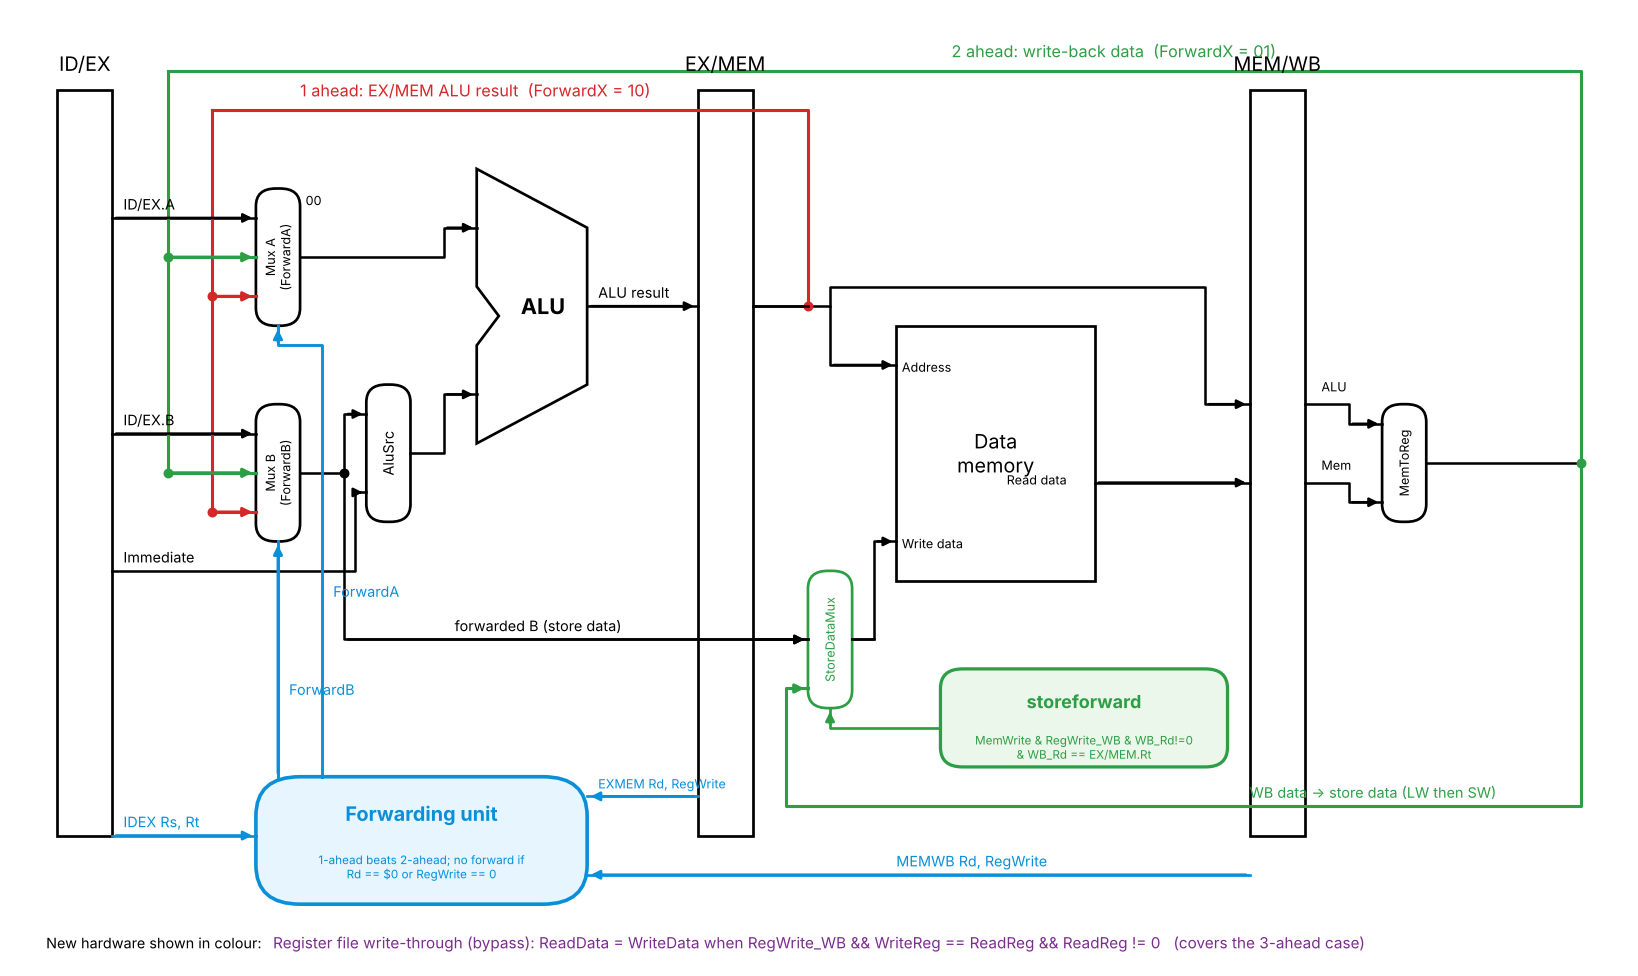
\includegraphics[width=\textwidth]{modified_datapath.png}
\caption{Modified datapath: forwarding muxes and unit, store-data forwarding, and register-file bypass.}\label{fig:dp}
\end{figure}

\section{Verification}
\code{fwd\_tb.v} runs the lab's 10 instructions plus the tests described above and checks the register file and data memory. All 14 checks pass. To confirm each feature is actually exercised, the following were disabled one at a time and the testbench was confirmed to fail in each case: the \code{\$0} guard, the RegWrite guard, the arbitration, the 2-ahead path, the register-file bypass, and the LW$\rightarrow$SW forward.

\begin{table}[H]\centering
\begin{tabular}{lll}\toprule
Feature & Test & Result\\\midrule
1 ahead & \code{add}/\code{slt}/\code{sub} chain & R5=569, R6=1, R7=145\\
2 ahead & \code{add \$R8,\$R7,\$R2} & R8=237\\
\code{\$0} write & \code{add \$0,...; add \$R11,\$0,\$R10} & R11=5\\
No write & \code{sw; add \$R12,\$R2,\$R2} & R12=184\\
Bypass (3 ahead) & \code{addi; nop; nop; add} & R14=6\\
Arbitration & \code{addi; addi; add} on one register & R16=6\\
LW$\rightarrow$SW & \code{lw \$R17; sw \$R17} & Mem[20]=92\\
LW, nop, SW & \code{lw \$R18; nop; sw \$R18} & Mem[21]=92\\\bottomrule
\end{tabular}
\caption{Summary of tests (all pass).}
\end{table}

\section{Files changed or added}
\begin{itemize}[nosep]
  \item \code{CPU.v}: forwarding muxes and unit, store-data mux, EX/MEM Rt register
  \item \code{forwardingunit.v}, \code{storeforward.v}: new modules
  \item \code{RegFile.v}: bypass gated by RegWrite
  \item \code{pipecontrol.v}, \code{stallmux.v}: port width declarations made consistent
  \item \code{fwd\_tb.v}: new self-checking testbench
\end{itemize}
\end{document}
